\documentclass[conference]{IEEEtran}
\IEEEoverridecommandlockouts

\usepackage{cite}
\usepackage{amsmath,amssymb,amsfonts}
\usepackage{booktabs}
\usepackage{multirow}
\usepackage{array}
\usepackage{url}
\usepackage{balance}
\usepackage{graphicx}
\usepackage{xcolor}
\usepackage{hyperref}
\usepackage{fontspec}
\setmainfont{Times New Roman}
\usepackage{fancyhdr}
\hypersetup{hidelinks}
\renewcommand{\arraystretch}{1.12}
\sloppy

\fancypagestyle{ieeeheader}{%
  \fancyhf{}
  \fancyhead[L]{\fontsize{10}{12}\selectfont STUDENT SCIENTIFIC RESEARCH COMMUNICATION, VOLUME II, 2026}
  \fancyhead[R]{\fontsize{10}{12}\selectfont \thepage}
  \renewcommand{\headrulewidth}{0pt}
}

\title{A Unified PostgreSQL-Based Concurrency Control Mechanism for Appointment Slot Reservations in Digital Healthcare Systems}

\author{%
\IEEEauthorblockN{Trinh Van Vu, Nguyen Chi Thuan, and Huynh Nam}
\IEEEauthorblockA{\textit{Faculty of Information Technology, Industrial University of Ho Chi Minh City}\\
}
}
\begin{document}
\maketitle
\pagestyle{ieeeheader}
\thispagestyle{ieeeheader}

\begin{abstract}
Concurrent appointment booking through independent conventional and AI-assisted workflows can cause overbooking when both paths update the same appointment slot without a shared serialization mechanism. This study investigates this cross-workflow concurrency issue in NovaCare and proposes a unified PostgreSQL-based reservation mechanism. Instead of handling bookings through separate reservation logic, both paths use the same transaction protocol to acquire an explicit row-level lock on the target slot, recheck its availability, and apply a guarded counter update before inserting the appointment record. The approach was evaluated using direct service-level tests on PostgreSQL 16.14. In the baseline, both conflicting requests successfully reserved a capacity-one slot in all 30 cross-workflow trials, confirming the observed race condition. After the shared transaction path was implemented, exactly one request succeeded and the competing request was rejected in all 120 trials across four execution modes. No over-capacity state was observed. These results indicate that database-level row locking combined with guarded updates eliminated the observed cross-workflow overbooking condition under the tested workload. The findings are limited to the experimental fixtures and appointment-creation workflow and do not establish production-wide correctness across all lifecycle operations.
\end{abstract}
\vspace{0.5\baselineskip}
\begin{IEEEkeywords}
appointment scheduling, PostgreSQL, concurrency control, row-level locking, occupancy management
\end{IEEEkeywords}

\section{Introduction}
Scheduling appointments is a core pillar of any clinical platform. In real-world systems, the exact same doctor schedule can be exposed through different user interfaces: a patient might book directly via a scheduling grid, or they might arrive via an AI-guided pre-examination workflow. Even though these screens look different to the end user, they ultimately write to the exact same underlying time slots in the database.

The primary requirement is straightforward: active bookings must never exceed a slot's maximum capacity. Meeting this requirement becomes tricky when separate application modules check and update availability independently. Under high concurrency, two separate transactions can both see an open slot before either one finishes writing. If both increment the counter without synchronization, an overbooking occurs.

In this research, we look closely at this issue using NovaCare as our testbed. Initial code reviews revealed that the standard booking flow and the AI pre-examination flow were operating independently. Our baseline experiments recorded the race condition, where both paths successfully secured a single-slot capacity. This paper addresses a focused, testable question: can we route both booking channels through a single, database-controlled occupancy claim so that PostgreSQL serializes competing requests?

\section{Related Work}
\subsection{Database Concurrency Control}
Concurrency control coordinates transactions that access shared data. This study uses pessimistic row-level locking for a small, highly contended capacity record.

The mechanism evaluated here explicitly locks appointment-slot rows and applies a guarded update within one transaction. PostgreSQL documents \texttt{FOR UPDATE} as preventing conflicting modifications to selected rows until the transaction ends \cite{postgreslocking}, and documents transaction isolation separately \cite{postgresisolation}. The effective isolation level was not recorded; therefore, no isolation-level-specific claim is made.

\subsection{Healthcare Appointment Scheduling}
Healthcare scheduling research usually studies access, resource utilization, waiting time, and service capacity. Those planning questions provide context, but they do not directly evaluate the application-level race between two digital booking workflows that mutate one shared slot counter. This paper therefore limits its claim to that concurrency boundary.

\subsection{Research Gap}
The gap is the absence of one tested occupancy-claim protocol shared by distinct application workflows targeting the same capacity record. This paper asks whether a shared PostgreSQL transaction path removes the specific conventional-versus-AI overbooking behavior under a bounded workload.

\section{Problem Definition and Correctness Properties}
Let $S$ denote the set of appointment slots. For each slot $s\in S$, let $C_s$ be its configured capacity and $B_s$ be its stored occupancy counter. Let $O_s$ denote the number of reservations that the experiment's fixture and transaction logic recognize as occupying slot $s$. The fundamental capacity property is
\begin{equation}
0 \leq O_s \leq C_s, \qquad \forall s\in S.
\label{eq:capacity}
\end{equation}
The counter-consistency property for the tested creation paths is
\begin{equation}
B_s = O_s.
\label{eq:counter}
\end{equation}
The study uses these properties only as test oracles for E2. They are not a complete business definition of occupancy for the wider appointment lifecycle.

For a capacity-one slot, two competing creation requests $r_1$ and $r_2$ must not both commit a reservation. More generally, a successful claim is permitted only when the slot remains active, available, and below capacity at the point where the claim is serialized. A failed multi-slot claim must not leave a partial set of counter or membership updates.

\section{Unified Occupancy Control Mechanism}
\subsection{Design Overview}
During our implementation phase in NovaCare, we noticed that relying on separate application logic for conventional booking and AI pre-examination was the root cause of the overbooking bug. To fix this cleanly without introducing heavy distributed locks (such as Redis leases), we decided to centralize the authority directly inside PostgreSQL.

V1 introduces a shared occupancy-claim operation used by both conventional appointment creation and AI pre-examination appointment creation. The operation executes inside the caller's existing Prisma transaction. It is responsible for acquiring the slot locks, validating the locked slot state, and updating occupancy. Appointment creation and slot-membership writes remain in the same transaction so that a failure aborts the complete database operation.

The mechanism does not use Redis as a booking lock. PostgreSQL is the authority for slot capacity in this prototype. This avoids introducing a separate lease-based coordination mechanism whose state would still need to be reconciled with the database transaction.

\subsection{Stable Lock Ordering}
For a request that occupies multiple slots, V1 sorts the slot identifiers before acquiring locks. Let $Q$ be the set of slot identifiers required by one appointment. The lock sequence is
\begin{equation}
q_1 < q_2 < \cdots < q_{|Q|},
\label{eq:lockorder}
\end{equation}
where $<$ is the stable ordering used by the implementation. Using the same order for competing multi-slot requests reduces the possibility of cyclic lock acquisition for this class of operation. It does not prove freedom from all deadlocks elsewhere in the application or database.

For each slot, the transaction executes a row lock equivalent to:
\begin{verbatim}
SELECT id, capacity, bookedCount, status,
       isActive, isAvailable
FROM appointment_slots
WHERE id = $1
FOR UPDATE;
\end{verbatim}
After the lock is acquired, the service rereads and validates the row. This post-lock validation is essential: a value observed before waiting for a lock may no longer represent the current state after the competing transaction commits.

\subsection{Guarded Occupancy Update}
A slot is eligible only if it remains active and available, has the expected available status, and has remaining capacity. The counter update is additionally guarded in the database. In abstract form, for slot $s$:
\begin{equation}
B_s \leftarrow B_s + 1
\quad\text{iff}\quad
B_s < C_s \land A_s \land V_s \land (T_s=\texttt{AVAILABLE}),
\label{eq:guard}
\end{equation}
where $A_s$ and $V_s$ represent the active and available flags, and $T_s$ is the slot status. The implementation uses a conditional SQL update with a predicate equivalent to the condition above and checks whether a row was returned/updated. A failed guard is treated as a booking conflict rather than a successful claim.

The claim operation is performed before appointment insertion. This ordering was selected after an initial smoke test exposed a deadlock in the earlier ordering, where appointment insertion preceded the counter update. The revised ordering avoids the observed lock-upgrade interaction in that smoke test. The initial smoke test was not part of the measured trial set.

\subsection{Atomic Multi-Slot Creation}
For an appointment requiring multiple consecutive slots, V1 claims every required slot within the same database transaction. It then creates the appointment record, status history, and one membership row per occupied slot. Slot-status resolution is also performed within the transaction. The transaction boundary is therefore:
\begin{equation}
\mathcal{T}=L\cup V\cup C\cup A\cup H\cup M\cup R,
\label{eq:transaction}
\end{equation}
where $L$, $V$, $C$, $A$, $H$, $M$, and $R$ denote locking, validation, claiming, appointment insertion, history insertion, membership insertion, and slot-status resolution, respectively.
If any operation throws before commit, PostgreSQL rolls back the writes made by that transaction.

The AI pre-examination path was changed to use the same claim and membership operations. This closes the specific gap in which the AI path incremented the primary slot counter without creating the same membership representation used by the conventional path. The membership rows are created for the tested V1 path; the experiment does not establish a complete lifecycle for releasing or consuming those memberships.

\section{Experimental Methodology}
\subsection{Environment and Isolation}
The implementation details and V0/V1 trial outputs are preserved as internal experimental artifacts. The experiments used PostgreSQL 16.14 on isolated test databases; V1 targeted \texttt{127.0.0.1:55440}. Tests invoked NestJS service methods directly through Prisma and did not measure HTTP behavior.
\subsection{Business Process Under Test}
The tested business flow starts when a patient requests an appointment through either the conventional booking path or the AI pre-examination path. Both paths select the target appointment slot and pass the request to the shared occupancy claim. Inside one PostgreSQL transaction, the service locks the slot row, checks the current capacity and availability, and applies the guarded \texttt{bookedCount} update. If the claim succeeds, it creates the appointment and the corresponding \texttt{AppointmentSlotBooking} membership records before committing. If a required operation fails, the transaction rolls back the counter and related writes. The experiments covered this booking-and-claim flow, including concurrent requests and a selected multi-slot rollback point. Payment, cancellation, expiry, rescheduling, refund, and administrative status changes were outside the measured pipeline.
\textbf{Synthetic data generation.} The experiments used synthetic data generated by the test harness. Each run created a shared hospital, specialty, doctor, workplace, and medical service. New patients and appointment slots were created for each trial. All tested slots had a capacity of one, an initial booked count of zero, and an available status.

The harness created trial-specific user and patient-profile records; V1 AI scenarios additionally created a completed synthetic pre-examination session.

In the concurrent booking scenarios, two different patients attempted to book the same slot through the normal and AI-assisted booking paths. The requests were executed concurrently using \texttt{Promise.all}. For selected V1 scenarios, synchronization hooks were used to control the request order.

The harness generated identifiers using \texttt{crypto.randomUUID()} and used \texttt{Date.now()} for timestamps. No fixed random seed was used. Trial-specific records were newly created, but the harness did not clear previous records between trials. Separate databases were used for V0 and V1. No real patient data or AI-generated data was used.

The V0 and V1 source copies were isolated. Both recorded the same Prisma schema hash (prefix: \texttt{a5a45a82b6a6}). The V1 source snapshot was associated with branch \texttt{develop} and Git HEAD prefix \texttt{585dcd8db9d6}. Full hashes were retained in the experiment artifacts. The original working repository contained uncommitted changes and was preserved; it was not reset or overwritten. Three schema layers must be distinguished: the Prisma declared schema, the schema created by the ten repository migration directories, and the schema of the original synchronized experimental database. The V1 reports describe an empty disposable database with repository migrations followed by Prisma schema synchronization. The exact V1 synchronization command was not preserved in a direct terminal log, and no original PostgreSQL dump or catalog export remains. Therefore, the preserved V1 result is not an independently reproduced migration-only result and should not be presented as exact reconstruction of the original database.

The effective transaction isolation level of the test connections was not captured. The paper therefore reports the database version and observed transaction behavior without attributing the results to a specific isolation level.

\subsection{Test Scenarios}
The measured V0/V1 comparison included three principal scenario groups:
\begin{itemize}
  \item \textbf{E1:} two conventional create requests compete for one capacity-one slot.
  \item \textbf{E2:} one conventional create request competes with one AI pre-examination create request for the same capacity-one slot. V1 was also tested with controlled request ordering and a shared barrier.
  \item \textbf{E6:} a successful multi-slot reservation and a multi-slot transaction with an injected failure.
\end{itemize}
Only E2 is within this paper's experimental claim.

Each measured scenario used 30 independent repetitions unless otherwise stated. The V1 E2 family contained four execution modes: baseline concurrent start, normal-first controlled order, AI-first controlled order, and shared-barrier release. Each mode was repeated 30 times, giving 120 E2 trials. The separate E1 and E6 scenarios each contained 30 trials. The V1 fault-injection point occurred immediately after the first slot-counter update and before appointment and membership insertion.

\subsection{Metrics}
Correctness metrics included successful and conflicting service calls, over-capacity observations, negative counters, counter--membership mismatches, missing or extra membership rows, duplicate membership rows, and recognized database deadlock or serialization-conflict outcomes. For a set of measured call latencies $L=\{\ell_1,\ldots,\ell_n\}$, the mean is
\begin{equation}
\bar{\ell}=\frac{1}{n}\sum_{i=1}^{n}\ell_i.
\end{equation}
The median and 95th percentile were computed using the nearest-rank convention. Latency covered service-call execution only and excluded fixture setup and post-test database readback. V1 controlled-barrier and fault-injection trials were excluded from the comparable latency measurements.

\section{Experimental Results}
We evaluated our implementation using an isolated test harness running PostgreSQL 16.14 on our local development setup. By invoking our NestJS service methods directly with synthetic workloads, we ran controlled test suites to measure correctness under the tested concurrent contention scenarios. Our primary goal was to examine whether the shared locking mechanism removed the overbooking outcome observed in the preserved V0 artifact while maintaining atomic rollbacks during the tested interruption point.
\subsection{Correctness Under Single-Slot Contention}
Table~\ref{tab:e1} reports E1. Both versions completed one successful request and one expected conflict per trial. No over-capacity state was observed in either version for this same-workflow scenario.

\begin{table}[!t]
\caption{E1: Conventional Create Versus Conventional Create}
\label{tab:e1}
\centering
\footnotesize
\begin{tabular}{lrr}
\toprule
Metric & V0 & V1 \\
\midrule
Trials & 30 & 30 \\
Service calls & 60 & 60 \\
Successful calls & 30 & 30 \\
Conflict calls & 30 & 30 \\
Over-capacity observations & 0 & 0 \\
Negative counters & 0 & 0 \\
\bottomrule
\end{tabular}
\end{table}

\subsection{Cross-Workflow Contention}
The principal defect was recorded in E2. In the preserved V0 artifact, both the conventional and AI pre-examination requests succeeded in all 30 trials, despite the slot capacity being one. Each trial therefore produced an over-capacity outcome. In the preserved V1 artifact, the shared occupancy claim serialized the competing requests: exactly one succeeded and the other returned a conflict in all 120 trials across the four execution modes.

\begin{table}[!t]
\caption{E2: Conventional Create Versus AI Pre-Examination Create}
\label{tab:e2}
\centering
\footnotesize
\begin{tabular}{lrr}
\toprule
Metric & V0 & V1 \\
\midrule
Trials & 30 & 120 \\
Service calls & 60 & 240 \\
Successful calls & 60 & 120 \\
Conflict calls & 0 & 120 \\
Over-capacity trials & 30 & 0 \\
Counter/membership mismatch trials & 30 & 0 \\
\bottomrule
\end{tabular}
\end{table}

The four V1 E2 modes produced the following winner distribution. The controlled ordering behaved as expected, while the shared-barrier mode allowed either workflow to win.

\begin{table}[!t]
\caption{V1 E2 Winner Distribution by Execution Mode}
\label{tab:e2modes}
\centering
\footnotesize
\begin{tabular}{lrrr}
\toprule
Execution mode & Trials & Normal wins & AI wins \\
\midrule
Concurrent start & 30 & 0 & 30 \\
Normal-first & 30 & 30 & 0 \\
AI-first & 30 & 0 & 30 \\
Shared barrier & 30 & 16 & 14 \\
\bottomrule
\end{tabular}
\end{table}

The V1 result is a bounded correctness observation for the tested code path and fixture. It does not prove that every booking writer in the application uses the shared operation, nor that every lifecycle transition preserves occupancy.

\iffalse
\subsection{Multi-Slot Reservation and Rollback}
In the preserved V1 artifact, all 30 successful multi-slot reservation trials completed successfully. In a separate set of 30 fault-injection trials, the test harness raised an intentional failure after the first counter update. All 30 recorded transactions rolled back the affected counters and memberships, and no appointment or status-history record from the failed transaction remained.

\begin{table}[!t]
\caption{E6: Multi-Slot Reservation and Injected Failure}
\label{tab:e6}
\centering
\scriptsize
\resizebox{\columnwidth}{!}{%
\begin{tabular}{lrr}
\toprule
Metric & Successful run & Fault injection \\
\midrule
Trials & 30 & 30 \\
Successful commits & 30 & 0 \\
Intentional failures & 0 & 30 \\
Complete rollback & -- & 30/30 \\
Partial counter/membership state & 0 & 0 \\
\bottomrule
\end{tabular}
}%
\end{table}

The rollback result applies only to the injected point: after the first counter update and before appointment/membership insertion. It does not test failures at every possible point in the transaction.

\subsection{Aggregate V1 Integrity Checks}
Across the preserved V1 test suite (210 trials and 360 service calls), the final test inventory contained 180 appointments, 270 slots, and 210 membership rows. The recorded integrity checks found zero over-capacity observations, zero negative counters, zero counter--membership mismatches, zero missing or extra memberships, zero duplicate membership rows, and zero recognized database deadlocks or serialization conflicts. The 180 failed calls comprise 150 expected occupancy conflicts and 30 intentional fault-injection failures; they are not all unexpected errors.

\subsection{Latency Measurements}
Table~\ref{tab:latency} summarizes the available descriptive latency measurements. Values are in milliseconds. They are not a controlled performance benchmark and should not be interpreted as evidence that V1 is faster than V0.

\begin{table*}[!t]
\caption{Descriptive Service-Call Latency (Milliseconds)}
\label{tab:latency}
\centering
\footnotesize
\begin{tabular}{llrrrrr}
\toprule
Scenario & Version & Mean & P50 & P95 & Max & Notes \\
\midrule
E1 conventional/conventional & V0 & 49.08 & 45.66 & 70.41 & 139.54 & 30 repetitions \\
E1 conventional/conventional & V1 & 42.17 & 38.43 & 54.37 & 119.12 & 30 repetitions \\
E2 conventional/AI & V0 & 49.13 & 44.12 & 76.77 & 117.06 & Both requests succeeded \\
E2 conventional/AI & V1 & 22.03 & 19.70 & 39.81 & 44.94 & Baseline; one success, one conflict \\
E6 multi-slot success & V0 & 47.11 & 41.52 & 60.76 & 122.97 & 30 repetitions \\
E6 multi-slot success & V1 & 44.64 & 42.51 & 55.49 & 60.46 & 30 repetitions \\
V1 all measured calls & V1 & 40.83 & 35.40 & 84.66 & 119.12 & Mixed scenario aggregate \\
\bottomrule
\end{tabular}
\end{table*}

E2 latency is not an apples-to-apples comparison because V0 completed two successful booking calls while V1 completed one successful call and rejected the competing request. The aggregate V1 latency also combines a different scenario mix from V0. E1 and E6 differences are descriptive only; no confidence intervals, significance tests, or performance-improvement claims are made. No HTTP 5xx rate was measured because the experiment invoked service methods directly.

Figure~\ref{fig:latency} visualizes the same descriptive means reported in Table~\ref{tab:latency}. The E2 reduction should be read together with the different success/conflict composition, rather than as a performance gain. Figure~\ref{fig:overcapacity} shows the central correctness contrast: the V0 cross-workflow trials exceeded capacity in every repetition, whereas V1 did not.

\begin{figure}[!t]
\centering
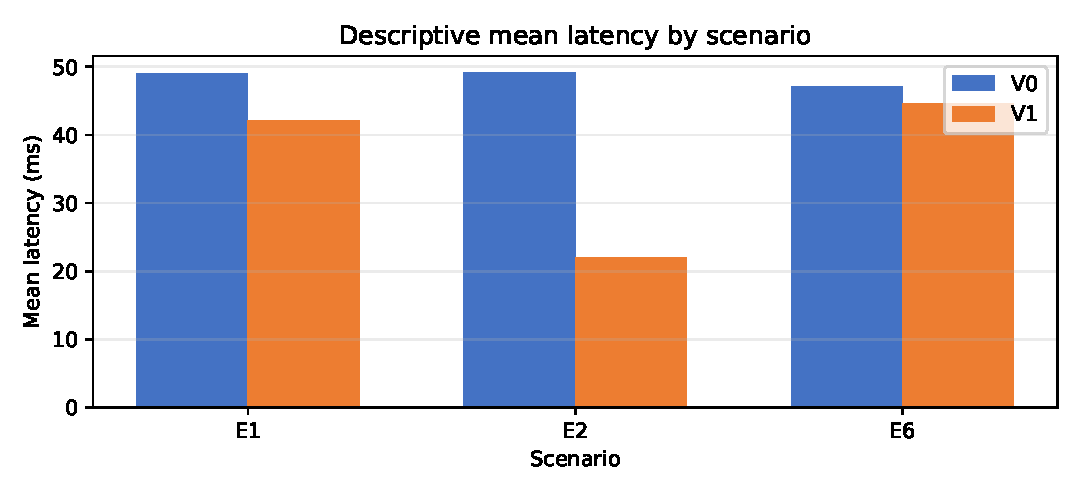
\includegraphics[width=\columnwidth]{img/latency_comparison.pdf}
\caption{Descriptive mean latency for E1, E2, and E6. Each pair is V0/V1 in milliseconds.}
\label{fig:latency}
\end{figure}

\begin{figure}[!t]
\centering
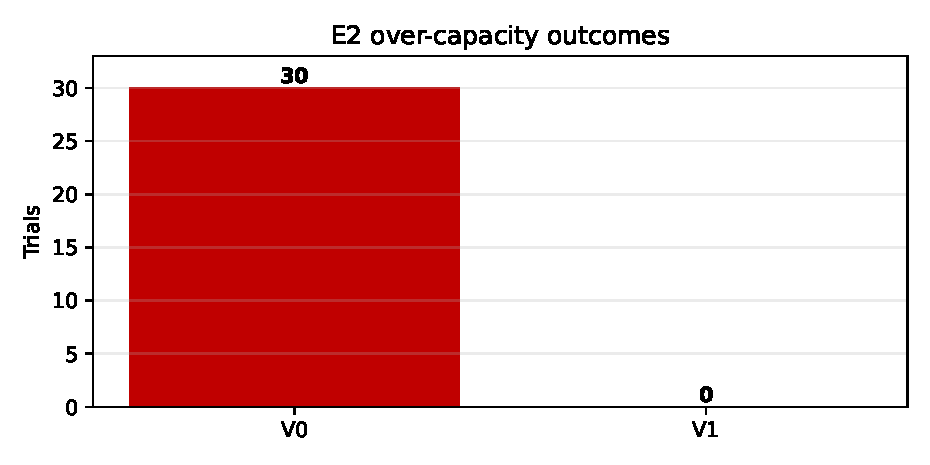
\includegraphics[width=\columnwidth]{img/overcapacity_comparison.pdf}
\caption{E2 over-capacity outcomes for the comparable 30-trial V0 baseline and the first 30-trial V1 concurrent-start mode.}
\label{fig:overcapacity}
\end{figure}
\fi

\section{Discussion}
The main result is the absence of the recorded cross-workflow overbooking outcome in the preserved V1 E2 trials. The preserved baseline allowed two distinct application paths to mutate the same capacity-one slot without a shared serialization point. V1 placed both paths behind the same PostgreSQL row-lock and guarded-update protocol. The database transaction then determined which request claimed the available capacity, while the competing request observed the updated state and failed with a conflict.

The multi-slot tests provide additional evidence for atomicity within the tested creation operation. Stable lock ordering reduces one common source of deadlock among transactions that request overlapping slot sets in the same order. The guarded update provides a second condition check at the write point rather than relying solely on an earlier application-level read. The transaction ensures that the tested counter and membership writes commit or roll back together.

These observations should be interpreted narrowly. The implementation does not establish a complete reservation lifecycle protocol. The broader source audit identified distinct paths for cancellation, rescheduling, expiry, payment callbacks, administrative status changes, and capacity edits. Those paths were not all routed through the V1 operation or tested in the reported experiment. The result therefore cannot be generalized to all appointment operations or all channels.

The experiment also does not establish multi-instance deployment behavior. PostgreSQL row locks are database-coordinated, but the test did not verify a production topology, external writers, worker replicas, or real payment-provider callbacks. The effective transaction isolation level was not recorded. The latency measurements are descriptive and confounded by different success/conflict outcomes in E2.

An initial one-repetition smoke test encountered a deadlock under an earlier write ordering. The implementation was changed to claim and update the slot counter before inserting the appointment. The smoke-test result was excluded from the measured dataset. This development iteration is reported to make the implementation history transparent; it is not presented as a measured deadlock-rate comparison.

\section{Threats to Validity and Limitations}
\subsection{Internal Validity}
The experiment used direct service invocations rather than HTTP requests. It therefore excludes network, controller, authentication, serialization, and client retry behavior. The experiment harness did not clear records between trials. Although each trial used newly created patients and appointment slots, previous records remained in the database. Therefore, the results should be interpreted within the tested experimental setup. The fixtures do not represent production traffic or real patient behavior. The transaction isolation level was not recorded, and latency statistics were not accompanied by confidence intervals or hypothesis tests. The exact V1 schema synchronization command was not preserved in a direct log, and no original database dump or catalog export remains.

\subsection{Construct Validity}
The occupancy oracle reflects the controlled test fixtures and V1 creation semantics. It is not a fully approved lifecycle definition for all appointment and payment states. The experiments do not determine whether completed or no-show appointments consume capacity, nor do they define expiry boundaries, grace periods, late-payment handling, refunds, or re-claim policy.

\subsection{External Validity}
The tests ran on one isolated PostgreSQL 16.14 environment with synthetic data. They do not represent production traffic, real patient behavior, multiple application instances, external hospital information systems, or payment-provider behavior. Results should not be generalized beyond the tested prototype and scenarios.

\subsection{Implementation Scope}
V1 changed selected source files in an isolated source copy and retained the same Prisma declared schema snapshot. The ten repository migrations did not, by themselves, reproduce all fields and models in that declared schema. The original synchronized database catalog is not available for exact reconstruction. Test-only hooks for barriers and fault injection were used in the harness and must be removed or replaced before any production adaptation. No production deployment or cutover was performed.

\section{Conclusion and Future Work}
This paper examined a concurrent booking defect in which conventional and AI pre-examination workflows could both reserve a capacity-one appointment slot. A unified PostgreSQL-based occupancy claim operation was implemented using stable row-lock ordering, post-lock rereading and validation, guarded counter updates, and transaction-scoped appointment and membership writes. In the preserved V1 artifact, the cross-workflow overbooking defect was not observed in 120 E2 trials, and all 30 injected multi-slot failures recorded rollback of the tested database writes. These observations are not an independent reproduction of the original environment; the exact V1 synchronization command and original database dump/catalog are unavailable.

The findings support the feasibility of a shared PostgreSQL transaction path for the specific creation workflows and test conditions studied. They do not establish correctness for the complete booking lifecycle, production deployment, distributed multi-instance topology, or performance superiority.

Future work should extend the same rigor to cancellation, rescheduling, expiry, payment callbacks, duplicate events, capacity changes, and administrative writers. These scenarios require an approved business truth table for occupancy and payment transitions before correctness can be judged. Subsequent experiments should record transaction isolation, database and connection-pool settings, raw trial artifacts, throughput, lock wait, retry behavior, and confidence intervals. A Redis-assisted variant should be considered only if measurements identify a concrete need beyond PostgreSQL's database-level coordination.

\balance
\balance
\begin{thebibliography}{6}
\bibitem{postgreslocking}
PostgreSQL Global Development Group, ``Explicit locking,'' \emph{PostgreSQL 16 Documentation}, Sec. 13.3. [Online]. Available: \url{https://www.postgresql.org/docs/16/explicit-locking.html}. Accessed: Nov. 9, 2026.

\bibitem{postgresisolation}
PostgreSQL Global Development Group, ``Transaction isolation,'' \emph{PostgreSQL 16 Documentation}, Sec. 13.2. [Online]. Available: \url{https://www.postgresql.org/docs/16/transaction-iso.html}. Accessed: Nov. 9, 2026.

\bibitem{v1impl}
NovaCare Research Team, ``V1 unified occupancy claim implementation report,'' internal technical artifact, 2026. Unpublished.

\bibitem{v0data}
NovaCare Research Team, ``V0 occupancy concurrency experiment results and raw trial data,'' internal experimental artifact, 2026. Unpublished.

\bibitem{v1data}
NovaCare Research Team, ``V1 occupancy concurrency experiment results and raw trial data,'' internal experimental artifact, 2026. Unpublished.
\end{thebibliography}

\end{document}
